%% chapter3_slides.tex
%% Beamer slides for Chapter 3: Efficiency -- E-values under the alternative hypothesis
%% "Hypothesis Testing with E-Values" by Aaditya Ramdas and Ruodu Wang (arXiv:2410.23614)
%% Reader-friendly style: intuition first, step-by-step derivations, worked numeric example
%% Compiled with: pdflatex -interaction=nonstopmode chapter3_slides.tex  (twice)
\documentclass[aspectratio=169,10pt]{beamer}

\usetheme{Madrid}
\usecolortheme{seahorse}
\usefonttheme{professionalfonts}

%% ── Packages ──────────────────────────────────────────────────────────────
\usepackage{amsmath,amssymb,amsfonts}
\usepackage{mathtools}
\usepackage{graphicx}
\usepackage{booktabs}
\usepackage{xcolor}
\usepackage{listings}

\graphicspath{{figures/}}

%% ── Python listing style ─────────────────────────────────────────────────
\lstdefinestyle{pycode}{
  language=Python,
  basicstyle=\ttfamily\scriptsize,
  numbers=left,
  numberstyle=\tiny\color{gray},
  frame=single,
  backgroundcolor=\color{gray!7},
  keywordstyle=\color{blue!70!black}\bfseries,
  commentstyle=\color{green!50!black}\itshape,
  stringstyle=\color{orange!80!black},
  showstringspaces=false,
  breaklines=true,
  tabsize=2,
  xleftmargin=1.5em,
  framexleftmargin=1.5em,
  aboveskip=4pt,
  belowskip=4pt,
}
\lstset{style=pycode}

%% ── Metadata ─────────────────────────────────────────────────────────────
\title[E-Values -- Ch.3]{Hypothesis Testing with E-Values}
\subtitle{Chapter 3: Efficiency -- E-values under the Alternative}
\author{Based on Ramdas \& Wang}
\date{}

\setbeamertemplate{footline}[frame number]
\setbeamertemplate{navigation symbols}{}

%% ── Macros ────────────────────────────────────────────────────────────────
\newcommand{\PP}{\mathbb{P}}
\newcommand{\QQ}{\mathbb{Q}}
\newcommand{\EE}{\mathbb{E}}
\newcommand{\RR}{\mathbb{R}}
\newcommand{\Scr}{\mathbb{S}}
\newcommand{\calP}{\mathcal{P}}
\newcommand{\calQ}{\mathcal{Q}}
\newcommand{\calF}{\mathcal{F}}
\newcommand{\calG}{\mathcal{G}}
\newcommand{\calX}{\mathcal{X}}
\newcommand{\indic}[1]{\mathbf{1}_{\{#1\}}}
\newcommand{\KL}[2]{\mathrm{KL}(#1 \,\Vert\, #2)}

\begin{document}

%% =========================================================================
\begin{frame}
  \titlepage
\end{frame}

%% =========================================================================
\begin{frame}{Where we are}
  \begin{itemize}
    \item \textbf{Chapter 2} asked: is my e-value \emph{valid}? ($\EE^\PP[E]\le 1$ under every null $\PP$.)
    \item \textbf{Chapter 3} asks: is my e-value \emph{any good}? I.e., under a true alternative $\QQ$, does $E$ actually get large?
    \item Validity is a \emph{safety} property (protects against false rejections). Efficiency is a \emph{power} property (rewards you when $H_1$ is true).
    \item Roadmap of this chapter:
    \begin{itemize}
      \item 3.1--3.2: powered tests/e-values/p-values, and when they exist at all;
      \item 3.3--3.4: the right way to measure ``how good'' -- \textbf{e-power};
      \item 3.5--3.6: the single best possible e-variable -- \textbf{log-optimality} and likelihood ratios;
      \item 3.7: how to approximate the best e-variable when the alternative is composite;
      \item 3.8: why $\EE^\QQ[\log E]$ is the \emph{only} reasonable notion of e-power.
    \end{itemize}
  \end{itemize}
\end{frame}

%% =========================================================================
\begin{frame}[allowframebreaks]{Notation you'll need}
  \begin{block}{Setup (recap from Ch.\ 1--2)}
    $\calP$ is the set of null distributions, $\calQ$ the set of alternative distributions. An \emph{e-variable} $E\ge 0$ satisfies $\EE^\PP[E]\le 1$ for every $\PP\in\calP$. A \emph{p-variable} $P$ satisfies $\PP(P\le t)\le t$ for every $t\in[0,1]$, every $\PP\in\calP$.
  \end{block}

  \begin{block}{Power of a test / powered e-variable (Definition 3.1)}
    The \emph{power} of a test $\phi\in[0,1]$ against $\QQ$ is $\EE^\QQ[\phi]$ (probability of correctly rejecting). A test $\phi$ is \emph{powered at level $\alpha$} against $\calQ$ if
    \[
      \EE^\PP[\phi]\le\alpha \ \text{ for every } \PP\in\calP, \qquad \EE^\QQ[\phi]>\alpha \ \text{ for every } \QQ\in\calQ.
    \]
    It is \emph{uniformly} powered if $\inf_{\QQ\in\calQ}\EE^\QQ[\phi]>\alpha$ (a single margin works for the whole alternative set). Likewise $E$ is a \emph{powered e-variable} against $\calQ$ if $\EE^\QQ[E]>1$ for every $\QQ\in\calQ$.

    \emph{Analogy:} think of $\phi$ as a smoke alarm. ``Powered'' means it rarely false-alarms (controlled by $\alpha$) \emph{and} it reliably goes off when there really is a fire (every $\QQ$).
  \end{block}

  \begin{block}{E-power (Definition 3.11) -- today's central new quantity}
    The \emph{e-power} of an e-variable $E$ against $\QQ$ is
    \[
      \EE^\QQ[\log E].
    \]
    Plain English: it is the \emph{expected growth rate, on a log scale}, of your evidence when the alternative $\QQ$ is really true. Since e-values are naturally \emph{multiplied} across independent experiments, the log turns multiplication into addition -- exactly like compound interest, where you track $\log(\text{wealth})$ to get a steady per-period growth \emph{rate}. Higher e-power $=$ your evidence compounds faster $=$ a better e-variable.
  \end{block}

  \begin{block}{Powered e-value/test, restated with e-power in mind}
    $E$ has \emph{positive e-power} against $\calQ$ if $\EE^\QQ[\log E]>0$ for every $\QQ\in\calQ$; \emph{uniformly} positive if $\inf_{\QQ\in\calQ}\EE^\QQ[\log E]>0$. Positive e-power is a \emph{stronger} requirement than being a powered e-variable ($\EE^\QQ[E]>1$), by Jensen's inequality (Section 3.3 below).
  \end{block}

  \framebreak

  \begin{block}{Log-optimality (Definition 3.18)}
    Comparing two e-variables $E_1,E_2$ for the same $\PP$ vs.\ simple $\QQ$: $E_1$ has \emph{greater e-power} than $E_2$ if $\EE^\QQ[\log(E_2/E_1)]\le 0$. An e-variable $E$ is \emph{log-optimal} if $\EE^\QQ[\log(E'/E)]\le 0$ for every other e-variable $E'$.

    \emph{Analogy:} among all legal betting strategies against a rigged coin, the log-optimal one is the \emph{Kelly bet} -- the one whose long-run bankroll growth rate cannot be beaten by any other strategy. Theorem 3.20 below shows this best strategy is simply the likelihood ratio $\mathrm{d}\QQ/\mathrm{d}\PP$.
  \end{block}

  \begin{block}{Kullback--Leibler (KL) divergence -- defined plainly}
    For distributions $\QQ,\PP$ with densities $q,p$ w.r.t.\ a common reference measure $\mathbb{L}$,
    \[
      \KL{\QQ}{\PP} \;:=\; \EE^\QQ\!\left[\log\frac{\mathrm{d}\QQ}{\mathrm{d}\PP}\right] \;=\; \int q(x)\log\frac{q(x)}{p(x)}\,\mathbb{L}(\mathrm{d}x).
    \]
    \textbf{Plain-English meaning:} $\KL{\QQ}{\PP}$ is the \emph{average log-likelihood-ratio} of $\QQ$ over $\PP$, when data really come from $\QQ$ -- a measure of \emph{how distinguishable $\QQ$ is from $\PP$}. It is always $\ge 0$ (Gibbs' inequality), and $=0$ exactly when $\PP=\QQ$ (indistinguishable). Bigger KL $=$ easier to tell $\QQ$ apart from $\PP$ $=$ faster evidence accumulation.
  \end{block}

  \begin{block}{Why this matters together}
    Theorem 3.20 (Section 3.5) shows: the log-optimal e-variable for simple $\PP$ vs.\ simple $\QQ$ is exactly the likelihood ratio $\mathrm{d}\QQ/\mathrm{d}\PP$, and its (best possible) e-power equals $\KL{\QQ}{\PP}$. This single fact will anchor our running numerical example.
  \end{block}
\end{frame}

%% =========================================================================
\begin{frame}{Section 3.1 -- Intuition: what does ``powered'' mean?}
  \begin{itemize}
    \item A test/e-variable is \emph{valid} if it rarely cries wolf under $H_0$.
    \item It is \emph{powered} if, in addition, it reliably flags $H_1$ when $H_1$ is true.
    \item Crucially: powered-ness is a property of a \emph{pair} $(\calP,\calQ)$. If the alternative $\calQ$ creeps arbitrarily close to the null $\calP$ (a ``boundary point''), no test or e-variable can be powered -- there is no way to reliably distinguish two hypotheses that are nearly identical.
  \end{itemize}
\end{frame}

\begin{frame}[allowframebreaks]{3.1 Powered tests, e-values, p-values}
  \begin{block}{Definition 3.1: powered tests and e-values}
    The \emph{power} of a test $\phi$ against $\QQ$ is $\EE^\QQ[\phi]$; the \emph{type-II error rate} is $1-$ power. Testing null $\calP$, a test $\phi$ is \emph{powered at level $\alpha\in(0,1)$} against $\calQ$ if
    \[
      \EE^\PP[\phi]\le \alpha \ \ \forall \PP\in\calP, \qquad \EE^\QQ[\phi]>\alpha \ \ \forall \QQ\in\calQ,
    \]
    and \emph{uniformly} powered if further $\inf_{\QQ\in\calQ}\EE^\QQ[\phi]>\alpha$. An e-variable $E$ is \emph{powered} against $\calQ$ if $\EE^\QQ[E]>1$ for every $\QQ\in\calQ$, and \emph{uniformly} powered if $\inf_{\QQ\in\calQ}\EE^\QQ[E]>1$.
  \end{block}

  \begin{exampleblock}{Example 3.3: when powered tests don't exist}
    Let $X_1,\dots,X_n$ be iid $N(\mu,1)$. Testing $H_0:\mu\le 0$ vs.\ $H_1:\mu>0$: the e-variable $\exp(X_1+\cdots+X_n-n/2)$ \emph{is} powered (though not uniformly). But testing $H_0:\mu<0$ vs.\ $H_1:\mu\ge 0$: \textbf{no} powered test or e-variable exists at all! The reason: $\mu=0$ is a boundary point shared in spirit by both sides, so nothing can have power there while staying valid arbitrarily close to it (proof uses Fatou's lemma to push a valid procedure at $\mu=-1/m$ through to the limit $\mu=0$).

    \emph{Takeaway (Remark 3.4):} if $H_0$ is an open set and $H_1$ is its exact complement, with continuous densities, powered procedures generically do not exist. Always leave an explicit gap around the boundary in practice.
  \end{exampleblock}

  \begin{block}{Definition 3.5: all-or-nothing e-variable}
    $E$ is \emph{all-or-nothing} if $E=\indic{A}/c$ for some event $A$ and constant $c>0$: it takes only the values $0$ or $1/c$. These are exactly the e-variables that come from ``hard'' binary tests.
  \end{block}

  \begin{block}{Fact 3.6: tests $\leftrightarrow$ bounded e-variables}
    For any $\alpha\in(0,1)$, there is a one-to-one correspondence between $[0,1/\alpha]$-valued e-variables and level-$\alpha$ tests, via
    \[
      E = \phi/\alpha.
    \]
    If $\phi$ is binary (reject iff a p-value $P\le\alpha$), the corresponding $E=\indic{P\le\alpha}/\alpha$ is all-or-nothing. \textbf{Consequence:} a powered level-$\alpha$ binary test exists iff a powered e-variable taking values in $\{0,1/\alpha\}$ exists -- e-values can always replicate what p-value tests do.
  \end{block}

  \begin{block}{Definition 3.7: powered p-values}
    For $\beta\in(0,1]$, a p-variable $P$ is \emph{powered on $[0,\beta]$} against $\calQ$ if $\QQ(P\le t)\ge t$ for all $t\in[0,\beta]$ (with strict inequality somewhere). It is \emph{powered} if this holds with $\beta=1$, meaning $P$ is strictly stochastically smaller than Uniform$[0,1]$ under every $\QQ\in\calQ$. In practice $\beta=0.25$ already suffices, since real rejections happen at small $\alpha$.
  \end{block}
\end{frame}

%% =========================================================================
\begin{frame}[fragile]{Python: powered vs.\ not-powered (Example 3.3)}
  \begin{lstlisting}
import numpy as np

def lr_evalue(x, mu):
    """Likelihood-ratio e-variable for H0: N(0,1) vs shift mu, n obs."""
    n = len(x)
    return np.exp(mu * x.sum() - n * mu**2 / 2)

rng = np.random.default_rng(0)
n = 50
# H1: mu > 0 strictly -- a powered e-variable exists, e.g. mu_hat = 1
mu_true = 1.0
reps = 20000
x = rng.normal(mu_true, 1, size=(reps, n))
E = np.array([lr_evalue(xi, 1.0) for xi in x])
print("mean E under Q (mu=1):", E.mean())        # > 1, as guaranteed
print("fraction E > 1/0.05 :", (E > 20).mean())  # power at level 0.05

# H0: mu < 0  vs  H1: mu >= 0 -- NO powered e-variable can exist
# (boundary point mu=0 is shared "in the limit" -- see Example 3.3 proof)
  \end{lstlisting}
  Running this confirms $\EE^\QQ[E]>1$ numerically -- but for the boundary-touching version of the problem, no choice of $E$ would ever give a uniform margin, however many observations we simulate.
\end{frame}

%% =========================================================================
\begin{frame}[allowframebreaks]{3.2 A unified existence result}
  \begin{block}{Assumption (U)}
    There exists $U\stackrel{d}{=}\mathrm{Unif}[0,1]$ under every $\PP\in\calP$ and $\QQ\in\calQ$, independent of everything else. (Very weak -- always satisfiable by ``lifting'' the sample space with an auxiliary coin flip.)
  \end{block}

  \begin{block}{Theorem 3.9: five equivalent notions of powered-ness}
    Under (U), for testing $\calP$ against $\calQ$ (no restriction), the following are equivalent:
    \begin{enumerate}
      \item[(i)] a bounded powered e-variable exists;
      \item[(ii)] a powered level-$\alpha$ test exists (for some/every $\alpha\in(0,1)$);
      \item[(iii)] a powered level-$\alpha$ \emph{binary} test exists (for some/every $\alpha$);
      \item[(iv)] a p-variable powered on $[0,\beta]$ exists (for some/every $\beta\in(0,1)$);
      \item[(v)] a powered p-variable exists.
    \end{enumerate}
  \end{block}

  \textbf{Intuition:} this is a ``no free lunch, no hidden extra power'' result. It says testability is testability, however you package it -- as a test, a bounded e-variable, or a p-variable. You cannot get more discriminating power by switching representations. (The directions (i)$\Leftrightarrow$(ii), (iii)$\Rightarrow$(i), (v)$\Rightarrow$(i) even hold without (U).)

  \begin{exampleblock}{Example 3.10: finite sample spaces are subtle}
    On a finite $\Omega$ with $\PP(\{\omega\})>0$ everywhere, testing $\PP$ vs.\ $\QQ\ne\PP$: a powered e-variable is simply the likelihood ratio $\QQ/\PP$. But \emph{no} p-variable can be powered on $[0,\beta]$ for any $\beta$ -- because any p-variable on a finite space takes only finitely many values, so $\QQ(P\le\alpha)=0$ for small enough $\alpha>0$, violating Definition 3.7. \textbf{Lesson:} e-variables can succeed where powered p-variables structurally cannot.
  \end{exampleblock}
\end{frame}

%% =========================================================================
\begin{frame}{Section 3.3 -- Intuition: why e-power, not just $\EE^\QQ[E]>1$?}
  \begin{itemize}
    \item ``Powered'' ($\EE^\QQ[E]>1$) only says the e-variable is valuable \emph{on average}, in raw (arithmetic) terms.
    \item But e-values are designed to be \emph{multiplied} across repeated/sequential experiments: $M_t = \prod_{s=1}^t E_s$.
    \item What matters for $M_t$'s long-run behavior is the average of $\log E_s$, not of $E_s$ -- exactly as in compound-interest/Kelly-betting problems.
    \item This motivates \textbf{e-power} $=\EE^\QQ[\log E]$: the exponential growth rate of your cumulative evidence.
  \end{itemize}
\end{frame}

\begin{frame}[allowframebreaks]{3.3 E-power and powered e-values}
  \begin{block}{Definition 3.11: e-power}
    The \emph{e-power} of $E$ against $\QQ$ is $\EE^\QQ[\log E]$ (assumed well-defined; it may equal $+\infty$ or $-\infty$). $E$ has \emph{positive e-power} against $\calQ$ if $\EE^\QQ[\log E]>0$ for each $\QQ\in\calQ$; \emph{uniformly} positive if $\inf_{\QQ\in\calQ}\EE^\QQ[\log E]>0$.
  \end{block}

  \begin{block}{Why the log? Connection to growth rate (Kelly criterion)}
    For iid e-variables $E_1,E_2,\dots$ with finite e-power, let $M_t=\prod_{s=1}^t E_s$, $t\in\mathbb{N}$. By the strong law of large numbers,
    \[
      \frac{\log M_t}{t} \;\xrightarrow{\ \QQ\text{-a.s.}\ }\; \EE^\QQ[\log E_1] \qquad (t\to\infty),
    \]
    i.e.\ the e-power \emph{is} the asymptotic growth rate of the cumulative e-process. This is exactly the classical Kelly criterion from betting/investment theory.
  \end{block}

  \begin{block}{Proposition 3.12: e-power controls power}
    Let $E_1,E_2,\dots$ be iid under $\QQ$, $M_t=\prod_{s=1}^t E_s$. If $\EE^\QQ[\log E_1]>0$, then $\QQ(M_t>1/\alpha)\to 1$ as $t\to\infty$, for every $\alpha>0$ (asymptotic power 1). If $\EE^\QQ[\log E_1]<0$, then $\QQ(M_t>1/\alpha)\to 0$ (asymptotic power 0).
  \end{block}

  \framebreak

  \begin{exampleblock}{Example 3.13: Gaussian e-power grows linearly in $n$}
    Testing $\PP=N(0,1)$ vs.\ $\QQ=N(\mu,1)$, $n$ iid observations. The likelihood-ratio e-value is
    \[
      E_n = \prod_{i=1}^n \exp(\mu X_i - \mu^2/2),
    \]
    with e-power $\EE^\QQ[\log E_n] = n\,\EE^\QQ[\mu X_1-\mu^2/2] = n\mu^2/2$: positive, and \emph{linear in $n$} -- more data means faster-growing evidence.
  \end{exampleblock}

  \begin{block}{Theorem 3.14: powered vs.\ positive e-power (they're closely related)}
    For nonnegative $X$ and any $\QQ$,
    \[
      \EE^\QQ[X]>1 \iff \EE^\QQ[\log(1-\lambda+\lambda X)]>0 \ \text{ for some } \lambda\in[0,1].
    \]
    So ``powered'' ($\EE^\QQ[X]>1$) is \emph{equivalent} to \emph{some soft-clipped version} of $X$ having positive e-power. Geometrically: $\EE^\QQ[\log E]>0$ means the \emph{geometric} mean of $E$ exceeds 1, a strictly stronger statement than the \emph{arithmetic} mean $\EE^\QQ[E]>1$ (Jensen's inequality). From any powered e-variable $E$, the shrunk version $1-\lambda+\lambda E$ (small $\lambda>0$) has positive e-power.
  \end{block}

  \begin{exampleblock}{Example 3.15: pathological gap between the two notions}
    Let $\Omega=\mathbb{N}_0$, $\PP=\tfrac12\delta_0+\tfrac12\delta_1$, $\calQ=\{\QQ_n\}$ with $\QQ_n = \tfrac1n\delta_n + (1-\tfrac1n)\delta_0$. Taking $E(n)=2n$ gives a \emph{uniformly powered, unbounded} e-variable ($\EE^\QQ_n[E]=2$ for all $n$), yet $\inf_n \EE^{\QQ_n}[\log(1-\lambda+\lambda E)]<0$ for every $\lambda$ -- and in fact \emph{no bounded} e-variable can even be powered here. Uniform power alone does not guarantee good (or even boundable) e-power.
  \end{exampleblock}

  \begin{exampleblock}{Example 3.16: e-power can mislead in the tails}
    Let $Y$ be Pareto(1) under $\QQ$ (infinite mean) and $E=\exp(6-Y/100)$. Then $\EE^\QQ[\log E] = -\infty$, yet $\QQ(E>100)>0.99$: $E$ gives very strong evidence with high probability, despite having ``the worst possible'' e-power. Moral: e-power is the right \emph{long-run, repeated-trial} criterion (Prop.\ 3.12), but is not the only lens for judging a single-shot e-value.
  \end{exampleblock}
\end{frame}

%% =========================================================================
\begin{frame}[fragile]{Python: e-power vs.\ raw power, simulated (Example 3.13)}
  \begin{lstlisting}
import numpy as np
rng = np.random.default_rng(1)

def simulate_epower(mu, n, reps=200000):
    X = rng.normal(mu, 1, size=(reps, n))
    logE = mu * X.sum(axis=1) - n * mu**2 / 2   # log of LR e-value
    return logE.mean(), np.exp(logE).mean()     # (e-power, plain E[E])

for n in [1, 10, 50, 100]:
    epow, meanE = simulate_epower(mu=0.3, n=n)
    print(f"n={n:4d}  e-power~{epow:7.3f}  (theory {n*0.3**2/2:7.3f})  "
          f"E[E]~{meanE:8.2f}")
  \end{lstlisting}
  Output confirms e-power $\approx n\mu^2/2$ growing \emph{linearly}, while the raw mean $\EE^\QQ[E]$ grows \emph{exponentially} in $n$ -- both say ``more data is better,'' but e-power is the additive, per-observation quantity that matches the Kelly growth-rate interpretation.
\end{frame}

%% =========================================================================
\begin{frame}[allowframebreaks]{3.4 Conditions for existence of powered e-variables}
  \begin{block}{Total variation (TV) distance}
    For distributions $\PP,\QQ$: $d_{\mathrm{TV}}(\PP,\QQ) = \sup_A |\PP(A)-\QQ(A)|$ (biggest possible probability gap on any event). For sets of distributions, $d_{\mathrm{TV}}(\calP,\calQ) = \inf_{\PP\in\calP,\QQ\in\calQ} d_{\mathrm{TV}}(\PP,\QQ)$: think of it as ``how close the nearest null scenario can get to the nearest alternative scenario.''
  \end{block}

  \begin{block}{Kraft--Le Cam theorem (background)}
    With a common reference measure: there is a test $\phi$ with a strict power/size gap $\inf_\QQ \EE^\QQ[\phi] - \sup_\PP\EE^\PP[\phi] > 2\varepsilon$ if and only if $d_{\mathrm{TV}}(\mathrm{Conv}(\calP),\mathrm{Conv}(\calQ)) > 2\varepsilon$ (convex hulls, in TV distance).
  \end{block}

  \begin{block}{Theorem 3.17: a checkable existence criterion}
    For testing $\calP$ against $\calQ$ with a common reference measure, TFAE:
    \begin{enumerate}
      \item[(i)] some test $\phi$ has $\inf_{\QQ\in\calQ}\EE^\QQ[\phi] > \sup_{\PP\in\calP}\EE^\PP[\phi]$;
      \item[(ii)] a uniformly powered \emph{bounded} e-variable exists for $\calP$ against $\calQ$;
      \item[(iii)] $d_{\mathrm{TV}}(\mathrm{Conv}(\calP),\mathrm{Conv}(\calQ)) > 0$.
    \end{enumerate}
  \end{block}

  \textbf{Intuition:} you can be uniformly powered (with a bounded e-variable, no less) \emph{if and only if} the convex hulls of your null and alternative scenario-sets are genuinely, positively separated in total variation. This turns an abstract testability question into a concrete geometric one about two convex sets of distributions. When $\calP,\calQ$ are finite, (iii) reduces to the two convex hulls simply being disjoint: $\mathrm{Conv}(\QQ_1,\dots,\QQ_M)\cap\mathrm{Conv}(\PP_1,\dots,\PP_L)=\varnothing$.
\end{frame}

%% =========================================================================
\begin{frame}{Running example, part 1: testing a coin's fairness}
  \begin{block}{Setup}
    $H_0: \theta=\theta_0=0.5$ (fair coin) \quad vs.\quad $H_1: \theta=\theta_1=0.7$ (biased coin).
    Observe $n$ iid flips $X_1,\dots,X_n\in\{0,1\}$ ($X_i=1$ for heads).
  \end{block}
  \begin{block}{The likelihood-ratio e-variable, one flip at a time}
    \[
      E_i \;=\; \frac{\theta_1^{X_i}(1-\theta_1)^{1-X_i}}{\theta_0^{X_i}(1-\theta_0)^{1-X_i}}
      \;=\; \Big(\tfrac{0.7}{0.5}\Big)^{X_i}\Big(\tfrac{0.3}{0.5}\Big)^{1-X_i}
      \;=\; 1.4^{X_i}\cdot 0.6^{1-X_i}.
    \]
    So $E_i = 1.4$ on heads, $E_i=0.6$ on tails -- and $E_n=\prod_{i=1}^n E_i$ over $n$ flips is a valid e-variable for $H_0$ (check: $\EE^{\theta_0}[E_i] = 0.5(1.4)+0.5(0.6)=1$, exactly).
  \end{block}
  \begin{block}{Step 1: e-power under the true alternative $\theta_1=0.7$}
    \[
      \EE^{\theta_1}[\log E_i] = 0.7\log(1.4) + 0.3\log(0.6) = 0.7(0.33647) + 0.3(-0.51083) = 0.08228.
    \]
    This equals $\KL{\mathrm{Bern}(0.7)}{\mathrm{Bern}(0.5)}=0.08228$ nats -- no coincidence (Sec.\ 3.5): the LR e-variable is log-optimal, with e-power always equal to the KL divergence.
  \end{block}
\end{frame}

%% =========================================================================
\begin{frame}{Section 3.5 -- Intuition: what's the \emph{best possible} e-variable?}
  \begin{itemize}
    \item For a simple null $\PP$ vs.\ simple alternative $\QQ$, classical (Neyman--Pearson) theory says the best \emph{test} thresholds the likelihood ratio $q(x)/p(x)$.
    \item Question: is there an analogous ``best e-variable''? Answer: yes, and it is even simpler -- it is \emph{exactly} the likelihood ratio itself, with no thresholding needed.
    \item Why? An e-variable just needs $\EE^\PP[E]\le 1$; the likelihood ratio $\mathrm{d}\QQ/\mathrm{d}\PP$ satisfies this with equality, and no other e-variable can have larger e-power.
  \end{itemize}
\end{frame}

\begin{frame}[allowframebreaks]{3.5 Log-optimality and likelihood ratios}
  \begin{block}{Definition 3.18: log-optimality (restated)}
    $E_1$ has greater (resp.\ equal) e-power than $E_2$ if $\EE^\QQ[\log(E_2/E_1)]\le 0$ (resp.\ $=0$). $E$ is \emph{log-optimal} if $\EE^\QQ[\log(E'/E)]\le 0$ for every other e-variable $E'$ -- i.e., no other e-variable can beat its e-power.
  \end{block}

  \begin{block}{Proposition 3.19: existence and uniqueness}
    For any $\calP$, a log-optimal e-variable against $\QQ$ always exists and is $\QQ$-almost-surely unique.
  \end{block}

  \begin{block}{Kullback--Leibler divergence, Eq.~(3.4)}
    \[
      \KL{\QQ}{\PP} := \EE^\QQ\!\left[\log\frac{\mathrm{d}\QQ}{\mathrm{d}\PP}\right] = \int q(x)\log\frac{q(x)}{p(x)}\,\mathbb{L}(\mathrm{d}x) \ \ (=\infty \text{ if } \QQ\not\ll\PP).
    \]
    \emph{Gibbs' inequality:} $\KL{\QQ}{\PP}\ge 0$ always, with equality iff $\PP=\QQ$.
  \end{block}

  \begin{block}{Theorem 3.20: THE key result of this section}
    For testing simple $\PP$ against simple $\QQ$ with $\QQ\ll\PP$: the ($\PP$-a.s.\ unique) log-optimal e-variable is the likelihood ratio $\mathrm{d}\QQ/\mathrm{d}\PP$. Its e-power equals $\KL{\QQ}{\PP}$ (possibly $\infty$).
  \end{block}

  \framebreak

  \begin{block}{Step-by-step: why the likelihood ratio wins}
    \textbf{Step 1.} Any exact e-variable can be written $E=\mathrm{d}\Scr/\mathrm{d}\PP$ for some distribution $\Scr\ll\PP$ (Proposition 2.12), and any e-variable is dominated by an exact one, so it suffices to compare exact e-variables.

    \textbf{Step 2.} It further suffices to take $\Scr\ll\QQ$ (else replace $\Scr$ by its $\QQ$-absolutely-continuous part; e-power is unaffected $\QQ$-a.s.).

    \textbf{Step 3.} Compare $E=\mathrm{d}\Scr/\mathrm{d}\PP$ against the likelihood ratio $\mathrm{d}\QQ/\mathrm{d}\PP$:
    \[
      \EE^\QQ\!\left[\log\frac{E}{\mathrm{d}\QQ/\mathrm{d}\PP}\right]
      = \int q(x)\log\!\left(\frac{s(x)/p(x)}{q(x)/p(x)}\right)\mathbb{L}(\mathrm{d}x)
      = -\int q(x)\log\frac{q(x)}{s(x)}\,\mathbb{L}(\mathrm{d}x) = -\KL{\QQ}{\Scr} \le 0,
    \]
    using Gibbs' inequality $\KL{\QQ}{\Scr}\ge 0$. \textbf{Conclusion:} $\mathrm{d}\QQ/\mathrm{d}\PP$ beats every candidate $E$, so it is log-optimal; equality holds only when $\Scr=\QQ$, giving uniqueness.
  \end{block}

  \begin{exampleblock}{Example 3.21: confirming optimality in the Gaussian case}
    Continuing Example 3.13: for $E_n(\theta)=\prod_i\exp(\theta X_i-\theta^2/2)$ (any fixed guess $\theta$, not necessarily $\mu$), the e-power under true $\QQ=N(\mu,1)^n$ is
    \[
      \EE^\QQ[\log E_n(\theta)] = n(\theta\mu - \theta^2/2).
    \]
    Maximizing over $\theta$: derivative $\mu-\theta=0 \Rightarrow \theta^\star=\mu$, confirming Theorem 3.20 -- guessing the \emph{true} mean shift is exactly optimal, with maximal e-power $n\mu^2/2 = n\cdot\KL{N(\mu,1)}{N(0,1)}$.
  \end{exampleblock}
\end{frame}

%% =========================================================================
\begin{frame}{Running example, part 2: log-optimality in numbers}
  \begin{block}{Step 1: the log-optimal e-variable IS the likelihood ratio}
    By Theorem 3.20, $E_i=1.4^{X_i}0.6^{1-X_i}$ (the LR e-variable from before) is log-optimal for $H_0:\theta=0.5$ vs.\ $H_1:\theta=0.7$, and its best-possible e-power equals
    \[
      \KL{\mathrm{Bern}(0.7)}{\mathrm{Bern}(0.5)} = 0.7\log\tfrac{0.7}{0.5}+0.3\log\tfrac{0.3}{0.5} = 0.08228 \text{ nats.}
    \]
  \end{block}
  \begin{block}{Step 2: a naive (suboptimal) e-variable}
    Suppose instead we guess a too-conservative alternative $\theta=0.6$:
    $E_i' = 1.2^{X_i}\cdot 0.8^{1-X_i}$. Its e-power under the true $\theta_1=0.7$ is
    \[
      \EE^{0.7}[\log E_i'] = 0.7\log(1.2)+0.3\log(0.8) = 0.7(0.18232)+0.3(-0.22314) = 0.06068 \text{ nats.}
    \]
  \end{block}
  \begin{block}{Step 3: compare growth over $n=100$ flips}
    Log-optimal: e-power $\times 100 = 8.228$, so $M_{100}\approx e^{8.228}\approx 3{,}740$.
    Naive: e-power $\times 100 = 6.068$, so $M_{100}\approx e^{6.068}\approx 432$.
    \emph{The log-optimal e-variable compounds nearly $9\times$ faster over 100 flips.}
  \end{block}
\end{frame}

%% =========================================================================
\begin{frame}{Figure: e-power in the coin example, three choices of $\theta$}
  \centering
  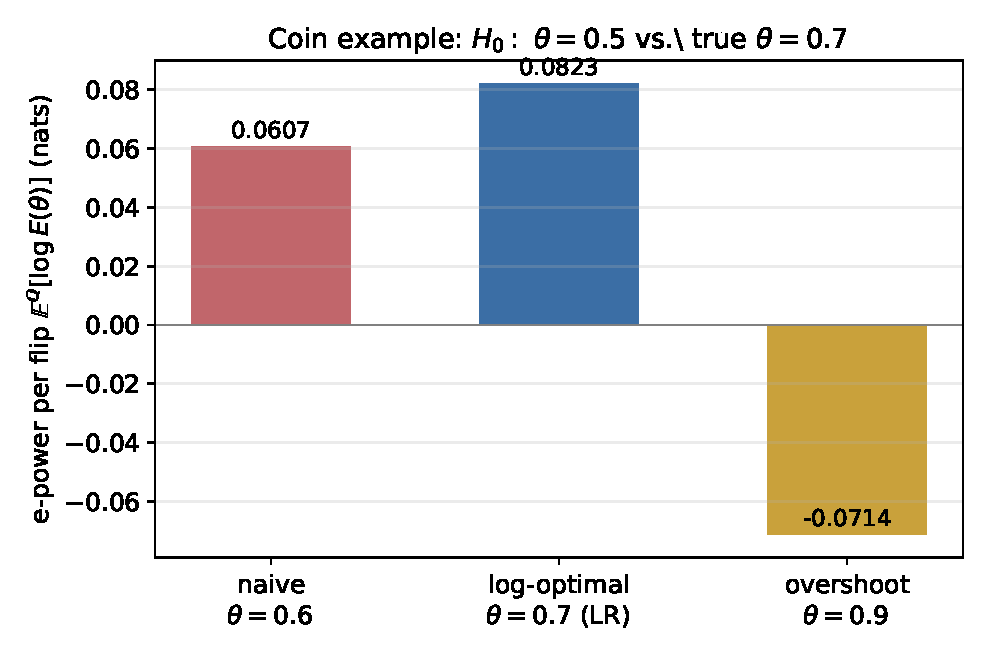
\includegraphics[width=0.62\linewidth]{fig_coin_epower_bar.pdf}\\
  \small Per-flip e-power $\EE^{\theta_1=0.7}[\log E(\theta)]$ for three assumed parameters $\theta$: the naive under-guess ($\theta=0.6$), the log-optimal true value ($\theta=0.7$), and an overshoot ($\theta=0.9$). The log-optimal choice always wins (Theorem 3.20).
\end{frame}

%% =========================================================================
\begin{frame}{Figure: e-power as a function of the assumed parameter}
  \centering
  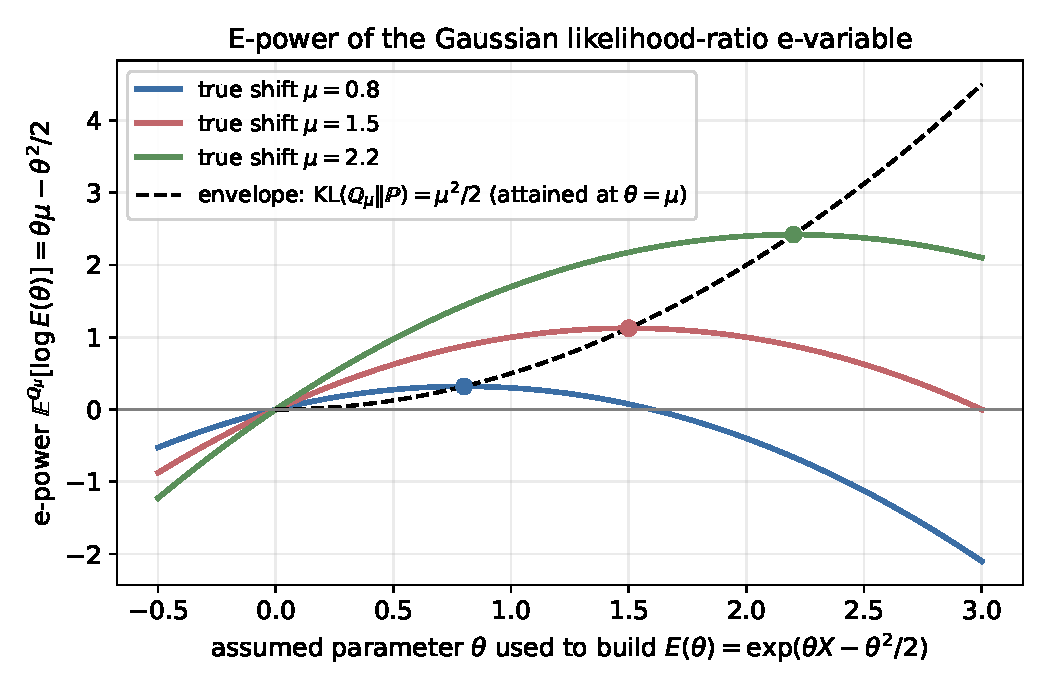
\includegraphics[width=0.62\linewidth]{fig_gaussian_epower.pdf}\\
  \small For the Gaussian LR e-variable $E(\theta)=\exp(\theta X-\theta^2/2)$ under true shift $\mu$: e-power $=\theta\mu-\theta^2/2$ peaks exactly at $\theta=\mu$ (dots), touching the KL envelope $\mu^2/2$ (dashed) -- a visual proof of Theorem 3.20 / Example 3.21.
\end{frame}

%% =========================================================================
\begin{frame}{Figure: growth rate over repeated coin flips}
  \centering
  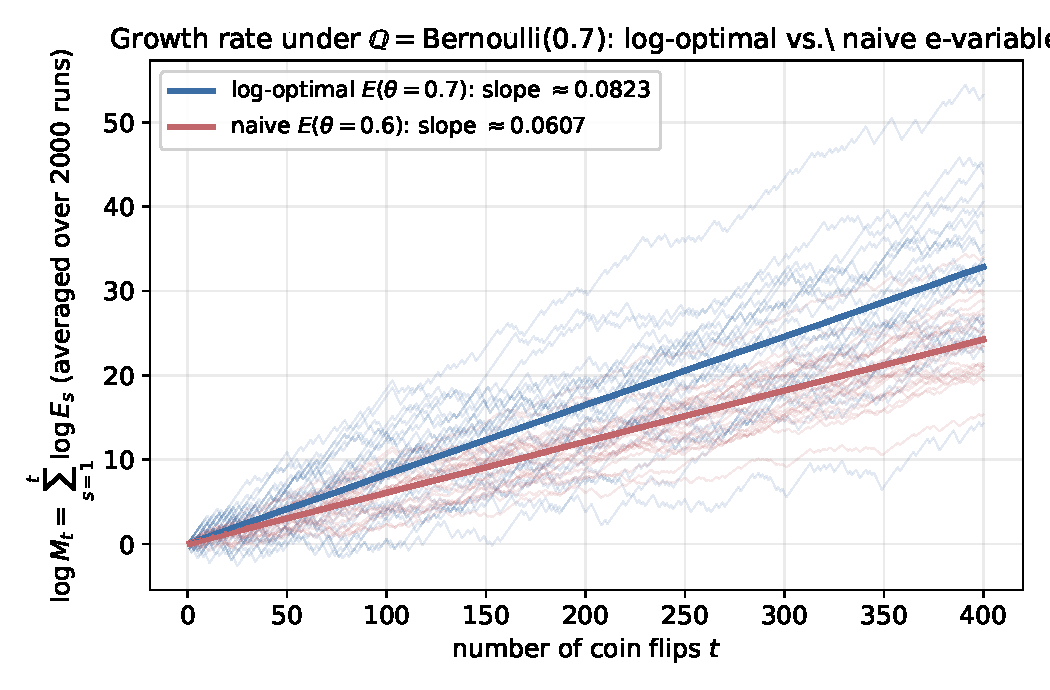
\includegraphics[width=0.62\linewidth]{fig_growth_paths.pdf}\\
  \small $\log M_t=\sum_{s\le t}\log E_s$ under the true $\QQ=\mathrm{Bernoulli}(0.7)$: log-optimal ($\theta=0.7$) climbs with slope $0.0823$, the naive choice ($\theta=0.6$) with slope $0.0607$ -- matching Proposition 3.12's growth-rate interpretation of e-power.
\end{frame}

%% =========================================================================
\begin{frame}[fragile]{Python: log-optimality \& KL divergence, from scratch}
  \begin{lstlisting}
import numpy as np

theta0, theta1_true, theta_naive = 0.5, 0.7, 0.6

def kl_bernoulli(q, p):
    """KL(Bernoulli(q) || Bernoulli(p)), in nats."""
    return q*np.log(q/p) + (1-q)*np.log((1-q)/(1-p))

epower_optimal = kl_bernoulli(theta1_true, theta0)          # = KL(0.7||0.5)
epower_naive   = kl_bernoulli(theta1_true, theta_naive)     # wrong-target LR

print(f"log-optimal e-power per flip : {epower_optimal:.5f} nats")
print(f"naive e-power per flip       : {epower_naive:.5f} nats")
print(f"ratio of growth after n=100  : "
      f"{np.exp(100*epower_optimal)/np.exp(100*epower_naive):.2f}x")
# -> log-optimal e-power per flip : 0.08228 nats
#    naive e-power per flip       : 0.06068 nats
#    ratio of growth after n=100  : 8.66x
  \end{lstlisting}
\end{frame}

%% =========================================================================
\begin{frame}[allowframebreaks]{3.6 Conditional log-optimality \& log-optimal calibrators}
  \begin{itemize}
    \item In practice, an e-variable must be computable from the \emph{observed data}, i.e.\ measurable w.r.t.\ some sub-$\sigma$-algebra $\calG\subseteq\calF$ (e.g.\ ``only the first $k$ of $n$ observations,'' or ``only a summary statistic'').
    \item We then want the e-variable that is log-optimal \emph{among those measurable w.r.t.\ $\calG$} -- not the unrestricted optimum, which may not be computable from what we observe.
  \end{itemize}

  \begin{block}{Proposition 3.22: conditional log-optimum = conditional likelihood ratio}
    If $\QQ\ll\PP$, the log-optimal e-variable w.r.t.\ $\calG$ exists ($\PP$-a.s.\ uniquely) and equals
    \[
      E = \frac{\mathrm{d}\QQ|_\calG}{\mathrm{d}\PP|_\calG} = \EE^\PP\!\left[\frac{\mathrm{d}\QQ}{\mathrm{d}\PP} \,\middle|\, \calG\right].
    \]
    \emph{In words:} restrict both distributions to what $\calG$ can see, take their likelihood ratio -- equivalently, average the full-information likelihood ratio over what $\calG$ doesn't know.
  \end{block}

  \begin{block}{Corollary 3.23: the log-optimal calibrator}
    Suppose $P$ is an exact p-variable ($\mathrm{Unif}[0,1]$ under $\PP$) for testing $\PP$ vs.\ $\QQ\ll\PP$, and $\EE^\PP[\mathrm{d}\QQ/\mathrm{d}\PP \mid P]$ is decreasing in $P$. Then the \emph{log-optimal calibrator} $f$ (recall: calibrators turn p-values into e-values) is
    \[
      f(P) = \EE^\PP\!\left[\frac{\mathrm{d}\QQ}{\mathrm{d}\PP} \,\middle|\, P\right], \qquad f\equiv 0 \text{ on } (1,\infty).
    \]
    \emph{Intuition:} among all calibrators (Ch.\ 2), this is the one specifically tuned to be best against a particular known alternative $\QQ$ -- it is the conditional expectation of the likelihood ratio given only the p-value.
  \end{block}
\end{frame}

%% =========================================================================
\begin{frame}{Section 3.7 -- Intuition: what if $\calQ$ isn't a single point?}
  \begin{itemize}
    \item Theorem 3.20 needs a \emph{simple} (single-distribution) alternative $\QQ$ to write down $\mathrm{d}\QQ/\mathrm{d}\PP$ explicitly.
    \item Real problems usually have a \emph{composite} $\calQ$ (e.g.\ ``some unknown $\theta_1\ne\theta_0$''). We can't build the log-optimal e-variable directly -- but we can get \emph{asymptotically} just as good, without ever committing to a single guess.
    \item Two practical recipes: \textbf{mixtures} (average over the likely alternatives) and \textbf{plug-in} (estimate the alternative as data arrive, one step at a time).
  \end{itemize}
\end{frame}

\begin{frame}[allowframebreaks]{3.7 Asymptotic log-optimality: mixtures and plug-in}
  \begin{block}{Goal: asymptotic log-optimality, Eq.~(3.6)}
    For a composite $\calQ$ (iid data, densities $p,q$ per observation), we want e-variables $E_n=E(X^n)$ such that for every $\QQ\in\calQ$,
    \[
      \lim_{n\to\infty} \frac{\EE^{\QQ^n}[\log E_n]}{n} \to \KL{\QQ}{\PP}.
    \]
    The right-hand side is the e-power of an all-knowing \emph{oracle} that is handed the true $\QQ$ in advance. Achieving this limit means our e-variable is (asymptotically) just as good as the oracle, without knowing $\QQ$ up front.
  \end{block}

  \begin{block}{Method 1: mixtures, Eq.~(3.7)}
    Pick a mixing (``prior'') distribution $\nu$ over $\calQ$, and define
    \[
      E_n = \int \prod_{i=1}^n \frac{q(X_i)}{p(X_i)}\,\nu(\mathrm{d}q).
    \]
    \textbf{Read the order carefully:} take the product of likelihood ratios \emph{first}, then mix. This is a valid e-variable (average of e-variables). It works whenever $\nu$ has full support over $\calQ$ and the mixture integral is tractable.
  \end{block}

  \begin{block}{Method 2: plug-in, Eq.~(3.8)}
    Let $\QQ_{i-1}\in\calQ$ be an estimate of the alternative based on only the first $i-1$ observations (e.g.\ the Bayes posterior mean under prior $\nu$), with density $q_{i-1}$. Define
    \[
      E_n = \prod_{i=1}^n \frac{q_{i-1}(X_i)}{p(X_i)}.
    \]
    Each factor is a ``one-step-ahead'' likelihood ratio using your current best guess; the product telescopes into a valid e-variable, and under mild conditions is asymptotically log-optimal whenever the corresponding mixture is.
  \end{block}

  \framebreak

  \begin{exampleblock}{Example 3.24: the t-test e-variable}
    $\calP=\{N(0,\sigma^2):\sigma>0\}$, $\calQ=\{N(\mu,\sigma^2):\sigma>0,\mu\ne0\}$. With $S_n=\sum X_i$, $V_n=\sum X_i^2$, for any $c>0$,
    \[
      \sqrt{\frac{c^2}{n+c^2}}\left(\frac{(n+c^2)V_n}{(n+c^2)V_n - S_n^2}\right)^{n/2}
    \]
    is a scale-invariant e-variable achieving (3.6). At $n=1$ it equals $1$ (zero e-power) -- one observation alone can never provide t-test evidence. Remarkably, a \emph{non-constant} e-variable with positive e-power at $n=1$ does exist: $E_1=|X_1|\exp((1-(X_1-a)^2)/2)$ for any fixed $a$, though it is not scale-invariant.
  \end{exampleblock}

  \begin{exampleblock}{Example 3.25: changepoint e-value}
    $n$ ordered observations; null: all iid $\PP$. Alternative: for some unknown $k\in[n]$, the last $k$ observations switch to a known $\QQ$ while the rest stay $\PP$. A natural \emph{mixture over the unknown changepoint} $k$ gives the e-value
    \[
      \frac{1}{n}\sum_{k=1}^n \prod_{i=n-k+1}^n \frac{q(X_i)}{p(X_i)}.
    \]
    This idea underlies the more general theory of \emph{e-detectors} for sequential change detection (beyond this book's scope).
  \end{exampleblock}
\end{frame}

%% =========================================================================
\begin{frame}[fragile]{Python: mixture method for a composite alternative}
  \begin{lstlisting}
import numpy as np
from scipy import integrate

# H0: theta = 0.5 (fair coin). H1: theta in (0.5, 1), unknown -- composite!
# Mixture e-value: integrate the likelihood ratio over a prior on theta.
theta0 = 0.5

def mixture_evalue(heads, n, prior_lo=0.5, prior_hi=1.0):
    def integrand(theta):
        # likelihood ratio for the whole sample, at this theta
        return (theta**heads * (1-theta)**(n-heads)) / \
               (theta0**heads * (1-theta0)**(n-heads))
    val, _ = integrate.quad(integrand, prior_lo, prior_hi)
    return val / (prior_hi - prior_lo)   # uniform mixing density = 1/(hi-lo)

rng = np.random.default_rng(2)
n, theta_true = 100, 0.7
heads = rng.binomial(n, theta_true)
E = mixture_evalue(heads, n)
print(f"heads={heads}/{n}, mixture e-value={E:.3g}, log E={np.log(E):.3f}")
# compare to the (unavailable in practice) oracle LR e-value at theta=0.7
  \end{lstlisting}
  Even without knowing $\theta_1=0.7$ in advance, the mixture e-value grows large -- illustrating asymptotic log-optimality without committing to a single alternative.
\end{frame}

%% =========================================================================
\begin{frame}{Section 3.8 -- Intuition: why $\EE^\QQ[\log E]$, and not something else?}
  \begin{itemize}
    \item So far we \emph{defined} e-power as $\EE^\QQ[\log E]$ and showed it behaves well. But is it the \emph{only} sensible choice, or just one of many?
    \item Section 3.8 shows: if you want a notion of ``how powerful is $E$'' that (a) scales sensibly when combined with prior evidence, and (b) agrees with the intuitive ``asymptotic power 1 vs.\ 0'' criterion of Proposition 3.12, then you are \emph{forced} into using (a strictly increasing transform of) $\EE^\QQ[\log E]$.
  \end{itemize}
\end{frame}

\begin{frame}[allowframebreaks]{3.8 Axiomatic justification of the e-power}
  \begin{block}{Setup}
    Let $\calX$ be nonnegative random variables bounded above and away from $0$ (technical convenience only). Fix an atomless $\QQ$. We study mappings $\Lambda^\QQ:\calX\to\RR$, candidates for ``e-power,'' \emph{without} requiring $E$ to be a valid e-variable for any specific $\calP$ -- e-power is a property of behavior under $\QQ$ alone. $\Lambda^\QQ(E_1)>\Lambda^\QQ(E_2)$ should mean ``$E_1$ is more powerful than $E_2$.''
  \end{block}

  \begin{block}{Axiom 3.26: Homogeneity}
    If $\Lambda^\QQ(E_1)\ge\Lambda^\QQ(E_2)$, then $\Lambda^\QQ(e_0 E_1)\ge \Lambda^\QQ(e_0 E_2)$ for any constant $e_0>0$.

    \emph{Motivation:} imagine a two-stage experiment where stage 1 already produced an e-value $e_0$. You must pick $E_1$ or $E_2$ for stage 2; the \emph{effective} comparison is really between $e_0E_1$ and $e_0E_2$. Homogeneity says your stage-2 ranking should not be overturned just by relabeling/rescaling by the (fixed, already-observed) $e_0$.
  \end{block}

  \begin{block}{Axiom 3.27: Asymptotic consistency}
    Let $(E_n)$, $(E_n')$ be iid sequences under $\QQ$. If $\Lambda^\QQ(E_1)\ge\Lambda^\QQ(E_1')$, then for every $\alpha\in(0,1)$,
    \[
      \QQ\Big(\textstyle\prod_{t=1}^n E_t' \ge \tfrac1\alpha\Big)\to 1 \implies \QQ\Big(\textstyle\prod_{t=1}^n E_t \ge \tfrac1\alpha\Big)\to 1.
    \]
    \emph{Motivation:} if the ``more powerful'' configuration by $\Lambda^\QQ$ is pitted against one that already achieves asymptotic power 1 when repeated, the more powerful one must too. This encodes Proposition 3.12's growth-rate intuition as an axiom.
  \end{block}

  \framebreak

  \begin{block}{Theorem 3.28: the representation theorem}
    $\Lambda^\QQ$ satisfies Axioms 3.26--3.27 \emph{if and only if}
    \[
      \Lambda^\QQ(E) = f\big(\EE^\QQ[\log E]\big), \qquad E\in\calX,
    \]
    for some strictly increasing $f$.
  \end{block}

  \textbf{Step-by-step proof sketch.}
  \begin{itemize}
    \item[\textbf{Step 1.}] Check $E\mapsto\EE^\QQ[\log E]$ itself satisfies both axioms (Axiom 3.27 via the strong law of large numbers); any strictly increasing transform of it therefore does too.
    \item[\textbf{Step 2.}] (Converse, by contradiction) Suppose $\Lambda^\QQ(E)>\Lambda^\QQ(E')$ but $\EE^\QQ[\log E]<\EE^\QQ[\log E']$. Rescale by a well-chosen $c>0$ (Axiom 3.26) so that $\log(cE)<0<\log(cE')$ in expectation.
    \item[\textbf{Step 3.}] Apply the strong law of large numbers to iid copies: $\log\prod cE_t\to-\infty$ but $\log\prod cE_t'\to+\infty$ in $\QQ$-probability -- i.e.\ the ``less powerful by $\Lambda^\QQ$'' sequence achieves asymptotic power 1 while the ``more powerful'' one achieves asymptotic power 0. This directly contradicts Axiom 3.27.
    \item[\textbf{Step 4.}] Hence $\Lambda^\QQ(E)>\Lambda^\QQ(E') \Rightarrow \EE^\QQ[\log E]\ge \EE^\QQ[\log E']$; a further tie-breaking argument (using Axiom 3.26 again, and monotonicity/bounded-variation of $c\mapsto\Lambda^\QQ(cE)$) upgrades this to strict inequality, showing $\Lambda^\QQ$ and $E\mapsto\EE^\QQ[\log E]$ induce the \emph{same ordering} -- hence the representation.
  \end{itemize}

  \begin{block}{Punch line}
    \textbf{If} you accept Axioms 3.26--3.27 as reasonable requirements for any sensible notion of ``e-power,'' \textbf{then} $\EE^\QQ[\log E]$ (up to relabeling by a strictly increasing $f$) is the \emph{only} possible choice. A natural such transform is the \emph{geometric mean} $\exp(\EE^\QQ[\log E])$: it is nonnegative, and exceeds $1$ exactly when e-power is positive.
  \end{block}

  \begin{block}{Proposition 3.29: sanity-check properties of $\Lambda^\QQ$}
    For an e-variable $E$: (i) $\Lambda^\QQ(E)>0 \Rightarrow \Lambda^\QQ(1-\lambda+\lambda E)>0$ for all $\lambda\in(0,1]$; (ii) same with ``$\ge 0$''; (iii) $\Lambda^\QQ(1-\lambda+\lambda E)$ is always well-defined for $\lambda\in[0,1]$; (iv) if $\Lambda^\QQ(E)<\infty$, then $\Lambda^\QQ(1-\lambda+\lambda E)\in\RR$ for all $\lambda\in[0,1]$. (Compare Theorem 3.14 -- shrinking $E$ towards 1 preserves the sign of e-power.)
  \end{block}
\end{frame}

%% =========================================================================
\begin{frame}{Chapter 3 summary}
  \begin{itemize}
    \item \textbf{Powered} tests/e-variables/p-variables (3.1) are unified by Theorem 3.9: any one form of testability gives you all the others (under mild conditions).
    \item \textbf{E-power} $\EE^\QQ[\log E]$ (3.3) is the right measure of ``how good'' an e-variable is for repeated/sequential use -- it is the asymptotic growth rate of cumulative evidence (Kelly criterion).
    \item Existence of powered procedures is checkable via a \textbf{total-variation separation} condition (3.4, Theorem 3.17).
    \item \textbf{Log-optimality} (3.5): for simple $\PP$ vs.\ simple $\QQ$, the best possible e-variable is exactly the \textbf{likelihood ratio}, and its e-power is exactly the \textbf{KL divergence} $\KL{\QQ}{\PP}$ (Theorem 3.20).
    \item When restricted to observable data (3.6), the log-optimal e-variable is a \textbf{conditional} likelihood ratio; this gives the log-optimal calibrator for p-values.
    \item For composite alternatives (3.7), \textbf{mixture} and \textbf{plug-in} constructions achieve the oracle's KL growth rate asymptotically, without knowing $\QQ$ in advance.
    \item The choice of $\EE^\QQ[\log E]$ as ``e-power'' is not arbitrary: it is the \emph{unique} (up to relabeling) notion satisfying two natural axioms (3.8, Theorem 3.28).
    \item \textbf{Running numeral:} testing a coin ($\theta_0=0.5$ vs.\ $\theta_1=0.7$), the log-optimal e-variable has e-power $\mathrm{KL}(0.7\|0.5)=0.0823$ nats/flip, versus $0.0607$ for a naive mis-targeted e-variable -- an $\approx 8.7\times$ faster-growing e-process after 100 flips.
  \end{itemize}
\end{frame}

\end{document}
